\section{Análisis de sensibilidad  de una monocapa como biosensor}
\label{section:sensLambda}

En las secciones anteriores se estudió la respuesta EM de una monocapa desordenada de NPs esféricas e idénticas, soportada por un sustrato con índice de refracción $n_s=1.5$, simulando a un vidrio BK7, e inmersa en agua (matriz con índice de refracción $n_m=1.33$). Cuando las NPs se iluminan en una configuración ATR, se observa un supuesto modo  plasmónico colectivo, el cual puede sintonizarse al seleccionar los siguientes parámetros: la fracción de cubierta $\Theta$ de la monocapa, el material de las NPs y el radio $a$ de éstas. En la Fig. \ref{fig:RT-AuAg} se muestran los resultados de la reflectancia de una monocapa de NPs de oro y una de NPs de plata, con los parámetros $a$ y $\Theta$ aptos para el sensado. La elección de $a=30$ nm y $\Theta=0.125$ para las NPs de oro, y $a=40$ nm y $\Theta=0.1$ para las de plata, sintoniza al supuesto modo  plasmónico colectivo dentro del espectro visible y, al calcular al reflectancia a las longitudes de onda $\lambda^{exc}$ que excitan al supuesto modo  plasmónico colectivo, la reflectancia es mínima ($R\approx 0$) para ángulos de incidencia menores a $80^\circ$ y para ambas polarizaciones. En esta sección se compara la respuesta EM de una monocapa desordenada de NPs de oro con arreglos nanoestrucuturados reportados en la literatura \cite{danilov2018ultra,svedendahl2009refractometric}; para una comparación entre una película continua de oro y de plata de $50$ nm (sensores comerciales) con las monocapas desordenadas de NPs esféricas de oro y de plata propuestas para el biosensado, consultar el apéndice \ref{section:A1}.

Los biosensores plasmónicos comerciales miden cambios en el índice de refracción de la matriz y su rendimiento puede cuantificarse mediante la sensibilidad de bulto $S_B$ \cite{estevez2014trends,svedendahl2009refractometric}, que es la dependencia del corrimiento $\delta \lambda^{exc}$ de la excitación ante cambios en el índice de refracción de la matriz $\delta n_m$ medido en unidades de índice de refracción (Refractive Index Units, RIU),\index{Índice de refracción!Unidades de índice de refracción RIU} es decir
%
	\begin{equation}
	S_B = \frac{\delta \lambda^{exc}}{\delta n_m}.
	\label{eq:SBulk}
	\end{equation}
%
Otro parámetro que caracteriza el rendimiento del biosensor es $\Gamma$, la anchura a media altura (Full Width at Half Maximum, FWHM)\index{Anchura a media altura (FWHM) ($\Gamma$)} de la reflectancia a la longitud de onda de la excitación. Para considerar tanto la sensibilidad de bulto como la FWHM en el rendimiento del biosensor, se define la \emph{figura de mérito} (Figure of Merit, FoM) de bulto  $\textit{FoM}_B$ dada por la expresión\index{Biosensor!Figura de Mérito (FoM)}\index{Biosensor!Figura de Mérito (FoM)!de bulto ($\textit{FoM}_B$)}
%
	\begin{equation}
	\textit{FoM}_B = \frac{S_B}{\Gamma}
			=\frac{1}{\Gamma}\frac{\delta \lambda^{exc}}{\delta n_m},
	\label{eq:FoM}
	\end{equation}
%
la cual se reporta evaluada en $n_m=1.33$. El empleo de la $\textit{FoM}_B$ permite tanto comparar la sensibilidad como calificar la calidad de biosensores ópticos que emplean distintos tipos de resonancias \cite{danilov2018ultra,svedendahl2009refractometric}, como puede ser la comparación entre sensores comerciales, basados en el plasmón polaritón de superficie (Surface Plasmon Polariton, SPP), el supuesto modo colectivo, predicho por del CSM, y los sensores basados en las resonancias de superfice localizadas (Localized Surface Plasmon Resonance, LSPRs), como las resonancias de una monocapa de nanodiscos desordenados \cite{svedendahl2009refractometric}, o las resonancias de red de superficie plasmónicas\footnote{Las PSLRs se excitan en arreglos periódicos de NPs cuando un haz difractado por la estructura, a su vez, excita una LSPR en un elemento de la red. Dado que las difracción del haz puede ser por la matriz o por el sustrato, los LSPRs se pueden acomplar con cada uno de estos medio y por tanto se identifican dos tipos de PSLRs \cite{danilov2018ultra}.} (Plasmon Surface Lattice Resonances, PSLRs), estudiadas en \cite{kabashin2009plasmonic} y \cite{danilov2018ultra}.

\begin{figure}[b!]\centering
	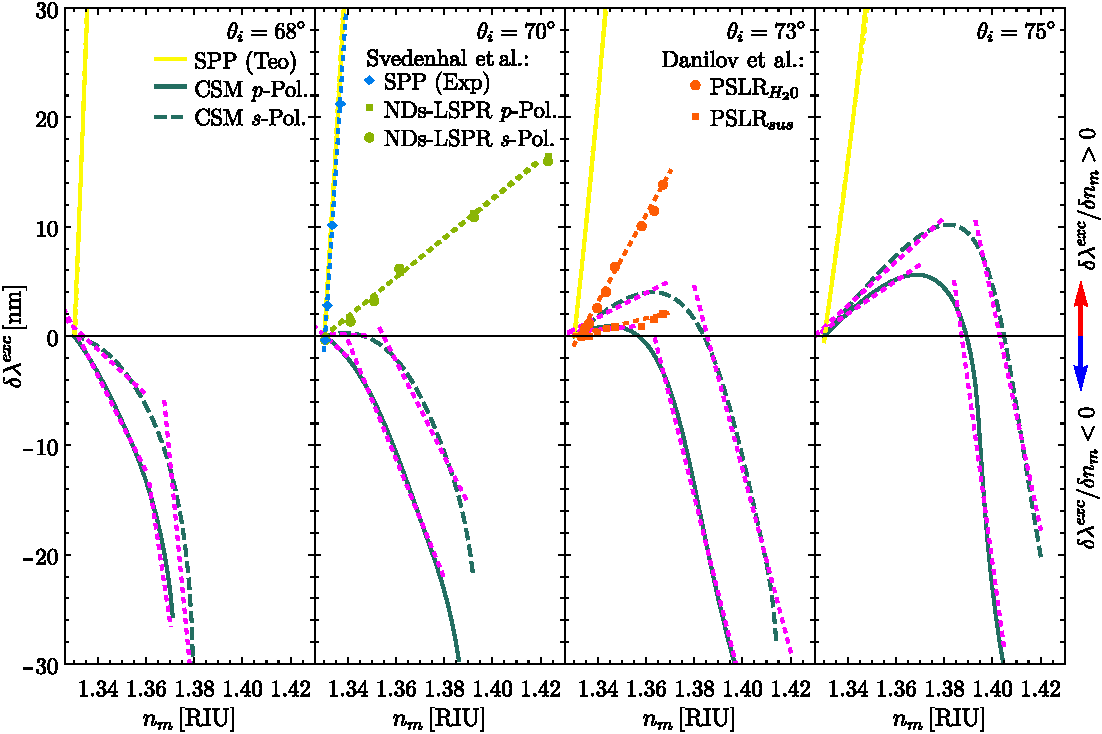
\includegraphics[width=\linewidth]{2-Resultados/figs/11-SPPCSM/1_comparacionAugtEye.pdf}\vspace*{-.7em}
	\caption{% Análisis de comportamiento del supuesto modo  plasmónico colectivo en una monocapa de NPs idénticas de oro ---radio $a=30$ nm y fracción de cubierta $\Theta=0.125$--- predicho por el CSM y  considerando $\theta_i=68^\circ,\, 70^\circ,\, 73^\circ$ y $75^\circ$.
Corrimiento al rojo de la longitud de onda de excitación $\delta\lambda^{exc}$ como función del índice de la matriz $n_m$, para el supuesto modo  plasmónico colectivo en una monocapa de NPs idénticas de oro ---radio $a=30$ nm y fracción de cubierta $\Theta=0.125$--- predicho por el CSM y  considerando $\theta_i=68^\circ,\, 70^\circ,\, 73^\circ$ y $75^\circ$ para polarización  \emph{p} (CSM \textit{p}-Pol., líneas turquesas continuas) y \emph{s} (CSM \textit{s}-Pol., líneas turquesas discontinuas), para el SPP en una película continua de oro de $50$ nm de grosor [SPP (Teo), líneas amarillas; SPP (Exp), rombos azules], la NDs-LSPR  en una monocapa desordenada de NDs para polarización \emph{p} (ND \textit{p}-Pol., cuadrados verdes) y \emph{s} (ND \textit{s}-Pol., círculos verdes) y el SPLR cuando se acopla con la matriz (PSLR$_{H_{2}O}$, puntos naranjas) y con el sustrato (PSLR$_{sus}$, cuadrados naranjas). Los datos experimentales del SPP y de las NDs-LSPR corresponden a los resultados de Svedenhal et al. reportados en \cite{svedendahl2009refractometric} y los de las PSLR a los resultados de Danilov et al. reportados en \cite{danilov2018ultra}. Cuando $S_B=\delta\lambda^{exc}/\delta n_m>0$ el modo se corre hacia el rojo y cuando $S_B<0$, se corre hacia el azul. Las líneas punteadas magenta, amarillas, verrdes y naranjas corresponden a aproximaciones lineales para determinar $S_B$ del supuesto modo plasmónico colectivo, el SPP (Teo) las NDs-LSPRs y las PSLR, respectivamente, y sus valores es encuentran en la tabla  \ref{tab:SB}.}\label{fig:SensThetai}
	\end{figure}	

En la Fig. \ref{fig:SensThetai} se compara la sensibilidad del supuesto modo  plasmónico colectivo de una monocapa de NPs de oro ($a=30$ nm y $\Theta=0.125$) con la del SPP (para un película de oro de $50$ nm de grosor), así como con resultados experimentales de la sensibilidad del SPP ---reportada por  Svedenhal et al.\footnote{\label{fn:Motivacion}Ver la Introducción para una descripción más detallada de sus resultados.} \cite{svedendahl2009refractometric} para una película de oro de $50$ nm de grosor a $\theta_i = 70^\circ$---, con resultados experimentales de la sensibildad de un  arreglo bidimensional desordenado de nanodiscos (NDs)---reportado por Svedenhal et al.\textsuperscript{\ref{fn:Motivacion}}  \cite{svedendahl2009refractometric}, donde los NDs son nanocilindros de oro de $30$ nm de altura y $120$ nm de diámetro, para polarización \emph{p} y \emph{s}, iluminados a $\theta_i = 70^\circ$---, que coincide con la LSPR de los NDs individuales (NDs-LSPR), y con resultados experimentales de la sensibildad de la PSLR ---reportada por Danilov et al.\textsuperscript{\ref{fn:Motivacion}} \cite{danilov2018ultra} para un arreglo ordenado cuadrado (parámetro de red de $134$ nm) de nanocilindros de oro de $90$ nm de altura y $134$ nm de diámetro a $\theta_i= 73^\circ$---. En la Fig. \ref{fig:SensThetai} se grafica el corrimiento $\delta\lambda^{exc}$ como función del índice de refracción de la matriz $n_m$, en un rango de $1.33$ RIU a $1.42$ RIU para los ángulos de incidencia $\theta_i = 68^\circ$, $70^\circ$, $73^\circ$ y $75^\circ$ para: el supuesto modo  plasmónico colectivo considerando polarización \emph{p} (CSM \textit{p}-Pol., líneas turquesas continuas) y \emph{s} (CSM \textit{s}-Pol., líneas turquesas discontinuas), una película de oro de $50$ nm de grosor [SPP (Teo), líneas amarillas; SPP (Exp), rombos azules], un arreglo desordenado de NDs  considerando polarización \emph{p} (NDs-LSPR círculos drados verdes) y la SPLR cuando el haz de luz se refracta por la matriz (PSLR$_{H_{2}O}$, puntos naranjas) y por el sustrato (PSLR$_{sus}$, cuadrados naranjas). La sensibilidad de bulto $S_B$ corresponde a la pendiente de las gráficas mostradas en la Fig. \ref{fig:SensThetai}. Las sensibilidades del SPP, de la NDs-LSPR y de la PSLR presentan un comportamiento lineal, mientras que el supuesto modo  plasmónico colectivo muestra una sensibilidad con una tendencia distinta. Para comparar las sensiblidades de las cuatro resonancias estudiadas, se aproximó a los datos experimentales del SPP, de la NDs-LSPR y a la PSLR una recta (líneas punteadas que se ajustan a cada conjunto de datos en la Fig. \ref{fig:SensThetai}) cuya pendiente es el valor de $S_B$, y para el supuesto modo  plasmónico colectivo predicho por el CSM se ajustó una recta (línea punteada magenta en la Fig. \ref{fig:SensThetai}) para distintos intervalos de $n_m$. Los resultados de la sensibilidad para el CSM, especificando el  intervalo de $n_m$ seleccionado, se  encuentran en la tabla \ref{tab:SB}, así como la sensibilidad del SPP para cada uno de los ángulos de incidencia, la de la NDs-LSPR a $70^\circ$ y la de la PSLR a $73^\circ$. A partir de la Fig. \ref{fig:SensThetai} se observa que el  CSM predice un corrimiento tanto al  rojo como al azul para el supuesto modo plasmónico colectivo, que corresponde a los valores de $S_B<0$ mostrados en la tabla \ref{tab:SB}.

%
\begin{table}[h!]
\centering
\caption{Resultados de sensibilidad $S_B$ del SPP, del supuesto modo  plasmónico colectivo predicho por el CSM (considerando una monocapa de NPs de oro)  para  los ángulos de incidencia $\theta_i = 68^\circ,\,70^\circ,\, 73^\circ$ y $75^\circ$, de la NDs-LSPR ($\theta_i=70^\circ$) y de la PSLR ($\theta_i=73^\circ$). Los valores de $S_B$ para el SPP corresponden a la pendiente de las líneas amarillas en  la Fig. \ref{fig:SensThetai}, en donde se consideró una película delgada de oro de $50$ nm de grosor, para la NDs-LSPR la pendiente de las líneas punteadas verdes que ajusta a los datos experimentales, y para la PSLR a la pendiente de las líneas punteadas naranjas que ajusta a los datos experimentales. Para el supuesto modo  plasmónico colectivo, la sensibilidad $S_B$ corresponde al ajuste lineal (líneas punteadas magentas en la Fig. \ref{fig:SensThetai} a un intervalo de $n_m$ seleccionado dado que $S_B$ no presenta un valor constante como sucede para las otras excitaciones. Datos experimentales extraídos de  \cite{danilov2018ultra} y \cite{svedendahl2009refractometric}.}\vspace*{-.7em}
\label{tab:SB}
\resizebox{\textwidth}{!}{%
\begin{tabular}{c|c|cc|cc}\hline\hline
			& SPP  & \multicolumn{2}{c|}{CSM \emph{p}-Pol.} & \multicolumn{2}{c}{CSM \emph{s}-Pol.}  \\
			& $S_B$ [nm RIU$^{-1}$] & \multicolumn{2}{c|}{[nm RIU$^{-1}$]} & \multicolumn{2}{c}{[nm RIU$^{-1}$]}   \\ \hline
\multirow{2}{*}{$\theta_i=68^\circ$}&\multirow{2}{*}{$6,142.79\pm 87.28$} & $-435.95\pm 6.94$   & $n_m \in (1.33,1.36)$  & $-204.96\pm 8.94$    & $n_m\in(1.33,1.36)$  \\
                                     &                                   & $\mathbf{-1,479.02\pm 99.32}$ & $\mathbf{n_m \in(1.36,1.39)}$  & $\mathbf{-2,275.10\pm 131.22}$ & $\mathbf{n_m\in(1.36,1.39)}$  \\ \hline
\multirow{2}{*}{$\theta_i=70^\circ$}&\multirow{2}{*}{$3,968.39\pm 52.43$} & $-201.85\pm 5.76$   & $n_m \in(1.33,1.34)$  & $-10.71\pm 5.16$     & $n_m\in(1.33,1.35)$  \\
                                    &                 & $-542.24\pm 8.05$   & $n_m \in(1.34,1.39)$  & $-435.23\pm 15.72$   & $n_m\in(1.5,1.39)$  \\ \hline
\multirow{2}{*}{$\theta_i=73^\circ$}& \multirow{2}{*}{$2,329.9\pm 37 .70$} & $20.75\pm 6.11$     & $n_m \in(1.33,1.35)$ & $111.20\pm 5.32$     & $n_m\in(1.33,1.37)$  \\
                                    &                                     & $-881.84\pm 10.05$  & $n_m \in(1.36,1.42)$  & $-833.11\pm 22.53$   & $n_m\in(1.38,1.42)$  \\ \hline
\multirow{2}{*}{$\theta_i=75^\circ$}& \multirow{2}{*}{$1,689.59\pm 18.11$} & $150.20\pm 4.56$    & $n_m \in(1.33,1.37)$  & $200.36\pm 4.55$     & $n_m\in(1.33,1.375)$ \\
                                     &                                     & $\mathbf{-1,613.37\pm 94.61}$ & $\mathbf{n_m \in(1.38,1.405)}$ & $\mathbf{-1,040.64\pm 35.02}$  & $\mathbf{n_m\in(1.38,1.42)}$\\ \hline\hline
 			& \multicolumn{3}{c|}{Svedenhal et al. \cite{svedendahl2009refractometric}} & \multicolumn{2}{c}{Danilov et al. \cite{danilov2018ultra}}        \\  \hline
			& 		SPP		&  	NDs-LSPR \emph{p}-Pol.	& NDs-LSPR \emph{s}-Pol. & PSRL$_{H_2O}$	& PSLR$_{H_2O}$ \\	
 			& $S_B$ [nm RIU$^{-1}$]& $S_B$ [nm RIU$^{-1}$] & $S_B$ [nm RIU$^{-1}$] & $S_B$ [nm RIU$^{-1}$] & $S_B$ [nm RIU$^{-1}$]\\	\hline
$\theta_i = 70^\circ$ & $3,423.96\pm 77.07$   &  $177.36\pm 6.52$ & $180.61\pm 3.70$ \\
$\theta_i = 73^\circ$ & 	  				&				& 			&              $397.11\pm 11.19$ &              $52.70\pm 6.03$ \\ \hline\hline
     \end{tabular}%
}
\end{table}
%

El valor de $S_B$ del SPP, de la NDs-LSPR y de la PSLR es constante para valores de $n_m$ entre $1.33$ RIU y $1.42$ RIU, además de ser positivo, es decir, que sólo se corre hacia el rojo al aumentar el valor de $n_m$. Por otro lado, la sensibilidad del supuesto modo  plasmónico colectivo varía según el valor de $n_m$ y presenta un corrimiento de la excitación tanto al rojo como al azul, como se observa en la Fig. \ref{fig:SensThetai}, siendo el corrimiento al azul (para $\theta_i\to\theta_c$) más sensible que el corrimiento al rojo. A partir de los resultados de la sensibilidad $S_B$ en la Fig. \ref{fig:SensThetai} y en la tabla \ref{tab:SB}, se concluye que  la sensibilidad del supuesto modo  plasmónico colectivo es comparable con la de la NDs-LSPR y la PSLR para algunos intervalos de $n_m$. Por ejemplo, para $\theta_i = 70^\circ$ el supuesto modo  plasmónico colectivo es más sensible que el arreglo de NDs para las dos polarizaciones cuando $1.35 \leq n_m \leq 1.39$ y para polarización \emph{p} en el intervalo $1.33\leq n_m \leq 1.35$, mientras que la monocapa de NDs es más sensible que el supuesto modo  plasmónico colectivo cuando $1.33\leq n_m \leq 1.35$ considerando polarización \emph{s}; para $\theta_i=73^\circ$ el supuesto modo  plasmónico colectivo es más sensible que la PSLR para $1.36\leq n_m \leq 1.42$  a ambas polarizaciones sin embargo, la PSLR es más sensible que el supuesto modo  plasmónico colectivo cuando $1.33\leq n_m \leq 1.36$.  A pesar de que el SPP es el más sensible de los modos presentados en la tabla \ref{tab:SB}, el supuesto modo plasmónico colectivo presenta valores de $S_B$ del mismo orden de magnitud cuando la excitación se corre al azul (ver datos en negritas en la tabla \ref{tab:SB}). Es decir, el arreglo desordenado de NPs esféricas compite en términos de sensibilidad con el arreglo nanoestructurado ordenado de cilindros y, para ángulos de incidencia cercanos al ángulo crítico, tiene una sensibilidad mayor.

Con base en los resultados de $S_B$ para el supuesto modo  plasmónico colectivo, se determinó que la longitud de onda de excitación $\lambda^{exc}$ de este modo puede correrse al rojo o al azul según el valor de $n_m$. Para visualizar este comportamiento, no presente para el SPP, la NDs-LSPR ni para la PSLR, se grafica en la Fig. \ref{fig:SensRpRs} la reflectancia de la monocapa de NPs de oro considerada en la Fig. \ref{fig:SensThetai} como función de la longitud de onda $\lambda$ para polarización \emph{p} (panel superior y líneas sólidas) y \emph{s} (panel inferior y líneas punteadas) para distintos valores de $n_m$: la opacidad de las curvas en la Fig. \ref{fig:SensRpRs} es proporcional al valor de $n_m$, siendo la línea más tenue el caso de $n_m=1.33$ y el más opaco el de $n_m=1.42$; se muestra en la Fig. \ref{fig:SensRpRs} el valor de $n_m$ máximo considerado para cada gráfica, por ejemplo, para $\theta_i=68^\circ$ se consideró desde $n_m=1.33$ hasta $1.390$, ya que el $\theta_c=\arcsin(1.390/1.5)\approx 68^\circ$. En la Fig. \ref{fig:SensRpRs} los puntos rojos corresponden a los mínimos en la reflectancia, es decir, a las longitudes de onda de excitación $\lambda^{exc}$ del supuesto modo plasmónico colectivo, mientras que las flechas negras son una ayuda al ojo para identificar el cambio en el valor de $\lambda^{exc}$ y de $R(\lambda^{exc})$ al aumentar el índice de refracción de la matriz.

\begin{figure}[h!]\centering
	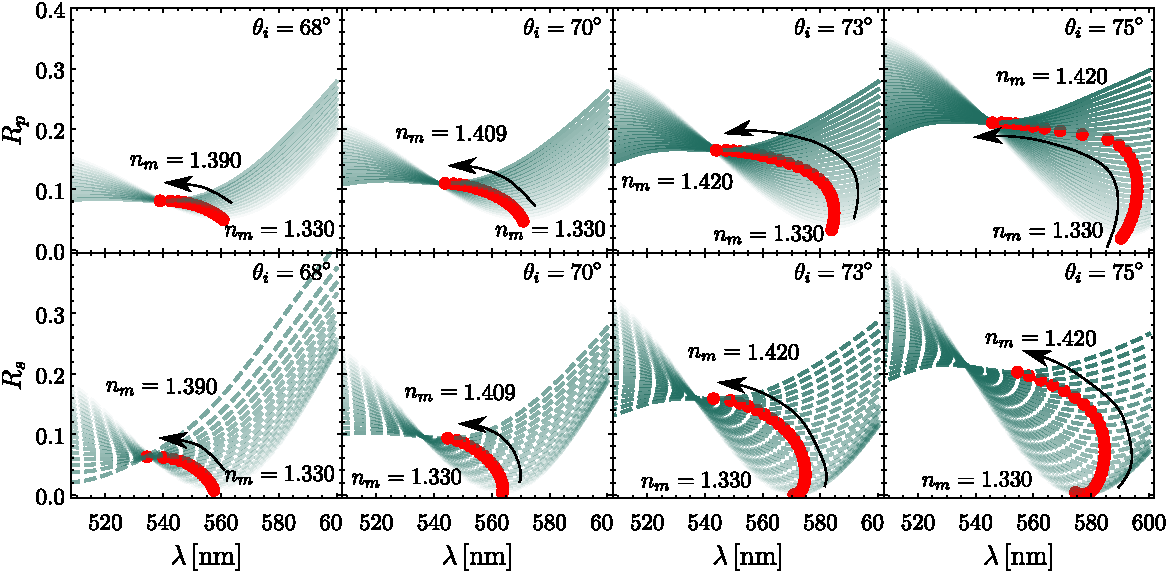
\includegraphics[width=1\linewidth]{2-Resultados/figs/11-SPPCSM/2-RpRs}\vspace*{-.7em}%
\caption{Reflectancia para polarización \emph{p}, $R_p$ (panel superior) y polarización \emph{s}, $R_s$ (panel inferior), de una monocapa desordenada de NPs de oro (radio $a=30$ nm y fracción de cubierta $\Theta=0.125$)  como función de la longitud de onda $\lambda$ para distinto valores del  índice de refracción de la matriz $n_m$. La opacidad de las gráficas es proporcional al valor de $n_m$  y los puntos rojos corresponden al mínimo de la reflectancia, es decir, al valor de $\lambda^{exc}$ considerado para los cálculos de la sensibilidad $S_B$ de la Fig. \ref{fig:SensThetai} y la tabla \ref{fig:SensRpRs}.	
	}\label{fig:SensRpRs}
	\end{figure}	

De la Fig. \ref{fig:SensRpRs} se observa que conforme el índice de refracción de la matriz aumenta, no sólo hay un corrimiento al rojo o al azul de la longitud de onda de excitación $\lambda^{exc}$  (puntos rojos en la Fig. \ref{fig:SensRpRs}) del modo colectivo,  sino también  el FWHM del supuesto modo  plasmónico colectivo aumenta. El supuesto modo  plasmónico colectivo es más sensible cuando, a un ángulo  $\theta_i$ fijo, éste se aproxima al ángulo crítico, es decir, cuando aumenta el valor de $n_m$ y se presenta un corrimiento al azul de $\lambda^{exc}$  sin embargo, es para estos casos que el FWHM aumenta, lo que puede dificultar la determinación experimental de $\lambda^{exc}$. Al considerar el valor de la FWHM, $\Gamma$, obtenido para la monocapa de oro, se calcula el valor de $\textit{FoM}_B$ para polarización \emph{p} y $\theta_i=68^\circ,\, 70^\circ,\, 73^\circ$ y $75^\circ$, dando como resultado  $\textit{FoM}_B= -2.64\pm0.07$ RIU$^{-1}$, $0.93 \pm0.07$ RIU$^{-1}$, $ \pm0.07$ RIU$^{-1}$ y $4.03\pm0.07$ RIU$^{-1}$, respectivamente, mientras que para \emph{s} $\textit{FoM}_B= 0.59\pm0.04$ RIU$^{-1}$, $1.88 \pm0.04$ RIU$^{-1}$, $ \pm0.04 $ RIU$^{-1}$ y $4.37\pm0.04$ RIU$^{-1}$, respectivamente. Los valores calculados de la FoM de bulto para el supuesto modo plasmónico colectivo son consistentes con los reportados en \cite{svedendahl2009refractometric} para arreglos nanoestructurados: del orden de la unidad.

Finalmente, para se calcula la longitud de penetración $\xi=1/k_x$, con $k_x$ la proyección paralela al la interfaz del matriz con el sustrato del vector de onda del supuesto modo plasmónico colectivo, mediante la siguiente expresión
%
\begin{equation}
\xi=\frac{1}{k_x}= \frac{\lambda^{exc}}{2\pi n_m}\frac{1}{\sin\theta_i}
\label{eq:penetracion}
\end{equation}
%
donde $\lambda^{exc}$ es la longitud de onda de excitación del supuesto modo colectivo al ángulo de incidencia $\theta_i$ excitado en la moncapa de NPs de oro con radio $a=30$ nm y $\Theta=0.125$  y en un intervalo de $n_m$ entre $1.33$ RIU y $1.42$ RIU. El valor de $\xi$ calculado fue de $\xi= (69.85\pm 2.97)$ nm para \emph{p} y $(70.39\pm 1.06)$ nm para \emph{s}, considerando $\theta_i=68^\circ$, y $(70.80\pm 1.27)$ nm para \emph{p} y $(70.59\pm0.82)$ nm con  $\theta_i=70^\circ$. Para $\theta=73^\circ$, se obtuvo que $\xi=(72.95\pm 0.79)$ nm para polarización \emph{p} y $\xi=(70.70\pm 0.48)$ nm y para $\theta_i=73^\circ$ mientras que $\xi=(72.48\pm0.43)$ nm para \emph{p} y $\xi=(70.72\pm 0.28)$ nm considerando $\theta_i=75^\circ$. El valor calculado de $\xi$ es aumenta para los ángulos de incidencia en los que la reflectancia toma valores más cercanos a cero,  es decir, que la longitud de penetración del supuesto modo colectivo modifica el valor de la reflectancia evaluada en $\lambda^{exc}$, lo que puede deberse a que el campo eléctrico que excita a las NPs de la monocapa interactúa en mayor medida con las NPs, lo que a su vez realza el fenómeno de esparcimiento múltiple y reduce la reflectancia. La longitud de penetración del supuesto modo plasmónico colectivo es aproximadamente $10$ nm  menor a la del SPP de una película continua de oro de $50$ nm (ver apéndice \ref{section:A1}), por lo que el supuesto modo plasmónico colectivo puede sensar cambios en el índice de refracción de la matriz a una distancia del sustrato comparable a la de lo sensores comerciales.


























